\documentclass[type=dr, dr=rernat, acm$^3$entcolor=tud7b,colorbacktitle, bigchapter, openright, twoside, 12pt ]{tudthesis}
%\documentclass[11pt,twoside,a4paper]{article}
\usepackage[english]{babel} 
\usepackage[utf8]{inputenc}
\usepackage{graphicx}
\usepackage{pstricks}
\usepackage{psfrag}
\usepackage{enumerate}
\usepackage{float}
\usepackage{epsfig}
\usepackage{geometry}
\usepackage{subfigure}
\usepackage{rotating}
\usepackage{minitoc}
\usepackage{multirow}
%\usepackage{appendix}

%%%% 1 1/2 facher Zeilenabstand:	
\usepackage{setspace}
\onehalfspacing




\begin{document}
\chapter{Patient Study}
\label{PatStudy}


\section{Introduction}

As described in section \textbf{REF} stereotactic body-radiation therapy with photons (SBRT) showed very promising results for treating non-small cell lung cancer (NSCLC) \cite{Baumann2009, Fakiris2009, Grutters2010, Ricardi2010, Timmerman2010, Greco2011}.
In chapter \textbf{REF} was showed that particle therapy (PT) can produce sharp dose gradients with a finite range of the beam and can thus provide higher healthy tissue sparing. 
This reduces both side effects as well as the risk of  secondary cancer \cite{Newhauser2011}. Treatment of lung tumors with PT is still challenging due to interplay and radiological path length changes (see section \textbf{REF}. 
Nevertheless, in recent years there have been several clinical studies using PT on lung tumors with promising results \cite{Tsujii2012}. It is important to note that all of these studies used passive beam 
scattering avoiding the problem of interplay between organ motion and scanning beam motion. However, the active beam scanning can provide even better dose shaping which becomes even more important in high dose single fractionation regimes. 
Therefore an in silico comparison between photon and active scanning ion carbon therapy (CiT) for NSCLC was conducted and will be presented in this chapter.
\newline
We hypothesize that 
(a) CiT could provide better healthy tissue sparing than photons in treating lung tumors or metastases due to its favorable dose profile.
(b) Patient characteristics can be identified that allow the selection of patients especially suited for CiT.
To evaluate our hypothesis, an in silico comparison of simulated CiT plans to single dose SBRT (SDRT) plans actually delivered was performed.
Target coverage and a wide range of OAR doses were assessed both with and without simulated motion on 4DCTs.  

\section{Materials and methods}

In this section input data will be presented as well as treatment planning parameters and procedures for SDRT and CiT. Finally, analysis method will be described.

\subsection{Patient data}

Study included 19 patients with in total 26 lesions that were actually treated with SDRT at the Funda\c{c}ao Champalimaud. The lesion size was 2.9 cm$^3$ (median, 25-75\% 1.4 - 9.7) and peak-to-peak motion was 3.1 mm (1.6 - 5.6).
Three patients had two targets, one had five and the rest one. 13 lesions were right-sided and 12 were left-sided and one was located in right cardiophrenic space. An overview of tumor characteristics can be found in Table~\ref{tab:paddata}.
Two computed tomographies (CT) were available for all patients. A planning CT was used for OAR delineation and SDRT planning. Target motion was estimated on a second, time-resolved CT (4D-CT), consisting of 10 motion phases. 
Clinical target volumes (CTV) were delineated using a registered positron emission tomography (PET) scan. The planning objectives were that 99 \% of planning target volume (PTV) must receive at least 24 Gy (D_{99}\% $\geq$ 24 Gy) 
in a single fraction, while all OAR constraints as defined in the AAPM task group 101 report on stereotactic radiotherapy had to be respected \cite{Benedict2010}. Different PTV definitions were used in SDRT and CiT, due to CiT sensitivity
to range changes. The definitions are described in next section.

\begin{table}[H]
  \centering
%   \footnotesize
  \caption{Lesion characteristics, with lesion locations, stages, peak-to-peak motions and volumes of corresponding CTV, SPTV and FTV. Abberevations for lesion location are: 
  RSL, right superior lung; IRL, inferior right lung; LSL, left superior lung; ILL, inferior left lung; RCS, right cardiophrenic space.}
  \begin{tabular}{|c|c|c|c|c|c|c|}
    \hline\hline
     & & & & \multicolumn{3}{|c|}{Volume (cm$^3$)} \\ \cline{5-7}
    \multirow{2}{*}{Number} & \multirow{2}{*}{Location} & \multirow{2}{*}{Stage} &
    Peak-to-peak & \multirow{2}{*}{CTV} & \multirow{2}{*}{SPTV} & \multirow{2}{*}{FTV}\\
     &  & & motion [mm] & & & \\
    \hline
    1 & LSL & IIa & 4.8 & 35.9 & 100 & 179 \\
    2 & LSL & Ia & 3.1 & 1.6 & 7.7 & 40.6 \\
    3 & IRL & IV & 12 & 2.3 & 11.6 & 32 \\
    4 & RSL & Ia & 0.5 & 6.9 & 25.2 & 38 \\
    5 & ILL & IV & 4.4 & 2.5 & 15 & 20.5 \\
    6 & ILL & IV & 7.5 & 1.4 & 7.7 & 26.5 \\
    7 & RSL & IV & 3.9 & 16 & 40 & 72.5 \\
    8 & ILL & IV & 0.6 & 139 & 261 & 255 \\
    9 & LSL & IV & 2 & 9.2 & 35 & 46.5 \\
    10 & IRL & IV & 3.4 & 10.2 & 38 & 45.5 \\
    11 & ILL & IV & 2.8 & 14.4 & 46.4 & 57.2 \\
    12 & ILL & IV & 5.8 & 3.8 & 17.4 & 23.4 \\
    13 & RSL & IV & 0.8 & 4.3 & 17.7 & 26.3 \\
    14 & LSL & IV & 3.4 & 2.7 & 14.5 & 23.1 \\
    15 & RSL & IV & 2.1 & 3.1 & 15.4 & 33.5 \\
    16 & LSL & IV & 0.5 & 0.5 & 5.4 & 6.7 \\
    17 & ILL & IV & 7.8 & 0.8 & 6.1 & 23.5 \\
    18 & LSL & IV & 0.1 & 1.7 & 15 & 23.5 \\
    19 & IRL & IIIb & 11.4 & 27 & 137 & 118.5 \\
    20 & RSL & Ia & 2.2 & 1.7 & 10 & 23.4 \\
    21 & RSL & IV & 0.2 & 0.9 & 3.2 & 14.9 \\
    22 & RSL & IV & 2.2 & 3.9 & 22.1 & 27.5 \\
    23 & LSL & IV & 3.1 & 9.8 & 28 & 51 \\
    24 & RSL & IV & 8.1 & 0.6 & 3.3 & 4.1 \\
    25 & LSL & IV & 1.4 & 0.8 & 5.9 & 10 \\
    26 & RCS & IV & 11.8 & 0.4 & 6.6 & 8.6 \\

    \hline\hline
  \end{tabular}
  \label{tab:patdata}
\end{table}

\subsection{Planning target volume definition}

To acm$^3$ount for range changes relevant for particles only, different PTV definitions were used for SDRT and CiT, as shown in Figure~\ref{Fig:PTV_def}. 
Within this thesis they will be named SPTV and FTV (field-specific target volume) for SDRT and CiT, respectively.
In SDRT, the responsible clinician determined the maximum breathing motion of the CTV from the 4DCT, hence creating an ITV. This ITV plus an additional 3 mm for setup uncertainty yielded the SPTV.

FTV was constructed following principles from Graeff et al \cite{Graeff2012}. Each beam has a unique FTV. For setup uncertainty margins of 3 mm laterally and 1 mm in beam's eyes view (BEV) were used on the CTV. 
Afterwards a water-equivalent path length ITV (WEPL-ITV) was build, using transformation maps from the B-Spline deformable registration of the 4DCT data \cite{Shackleford2010}. Additional 2 mm + 2 \% proximal and distal margins 
were added in BEV to acm$^3$ount for uncertainty from Hounsfield units to water equivalent path length conversion.

If the target overlapped with an OAR (e.g. small airways) then OAR plus a margin of 2-5 mm was subtracted from SPTV or FTV, to satisfy OAR constraints.

\begin{figure}[H]
\begin{center}
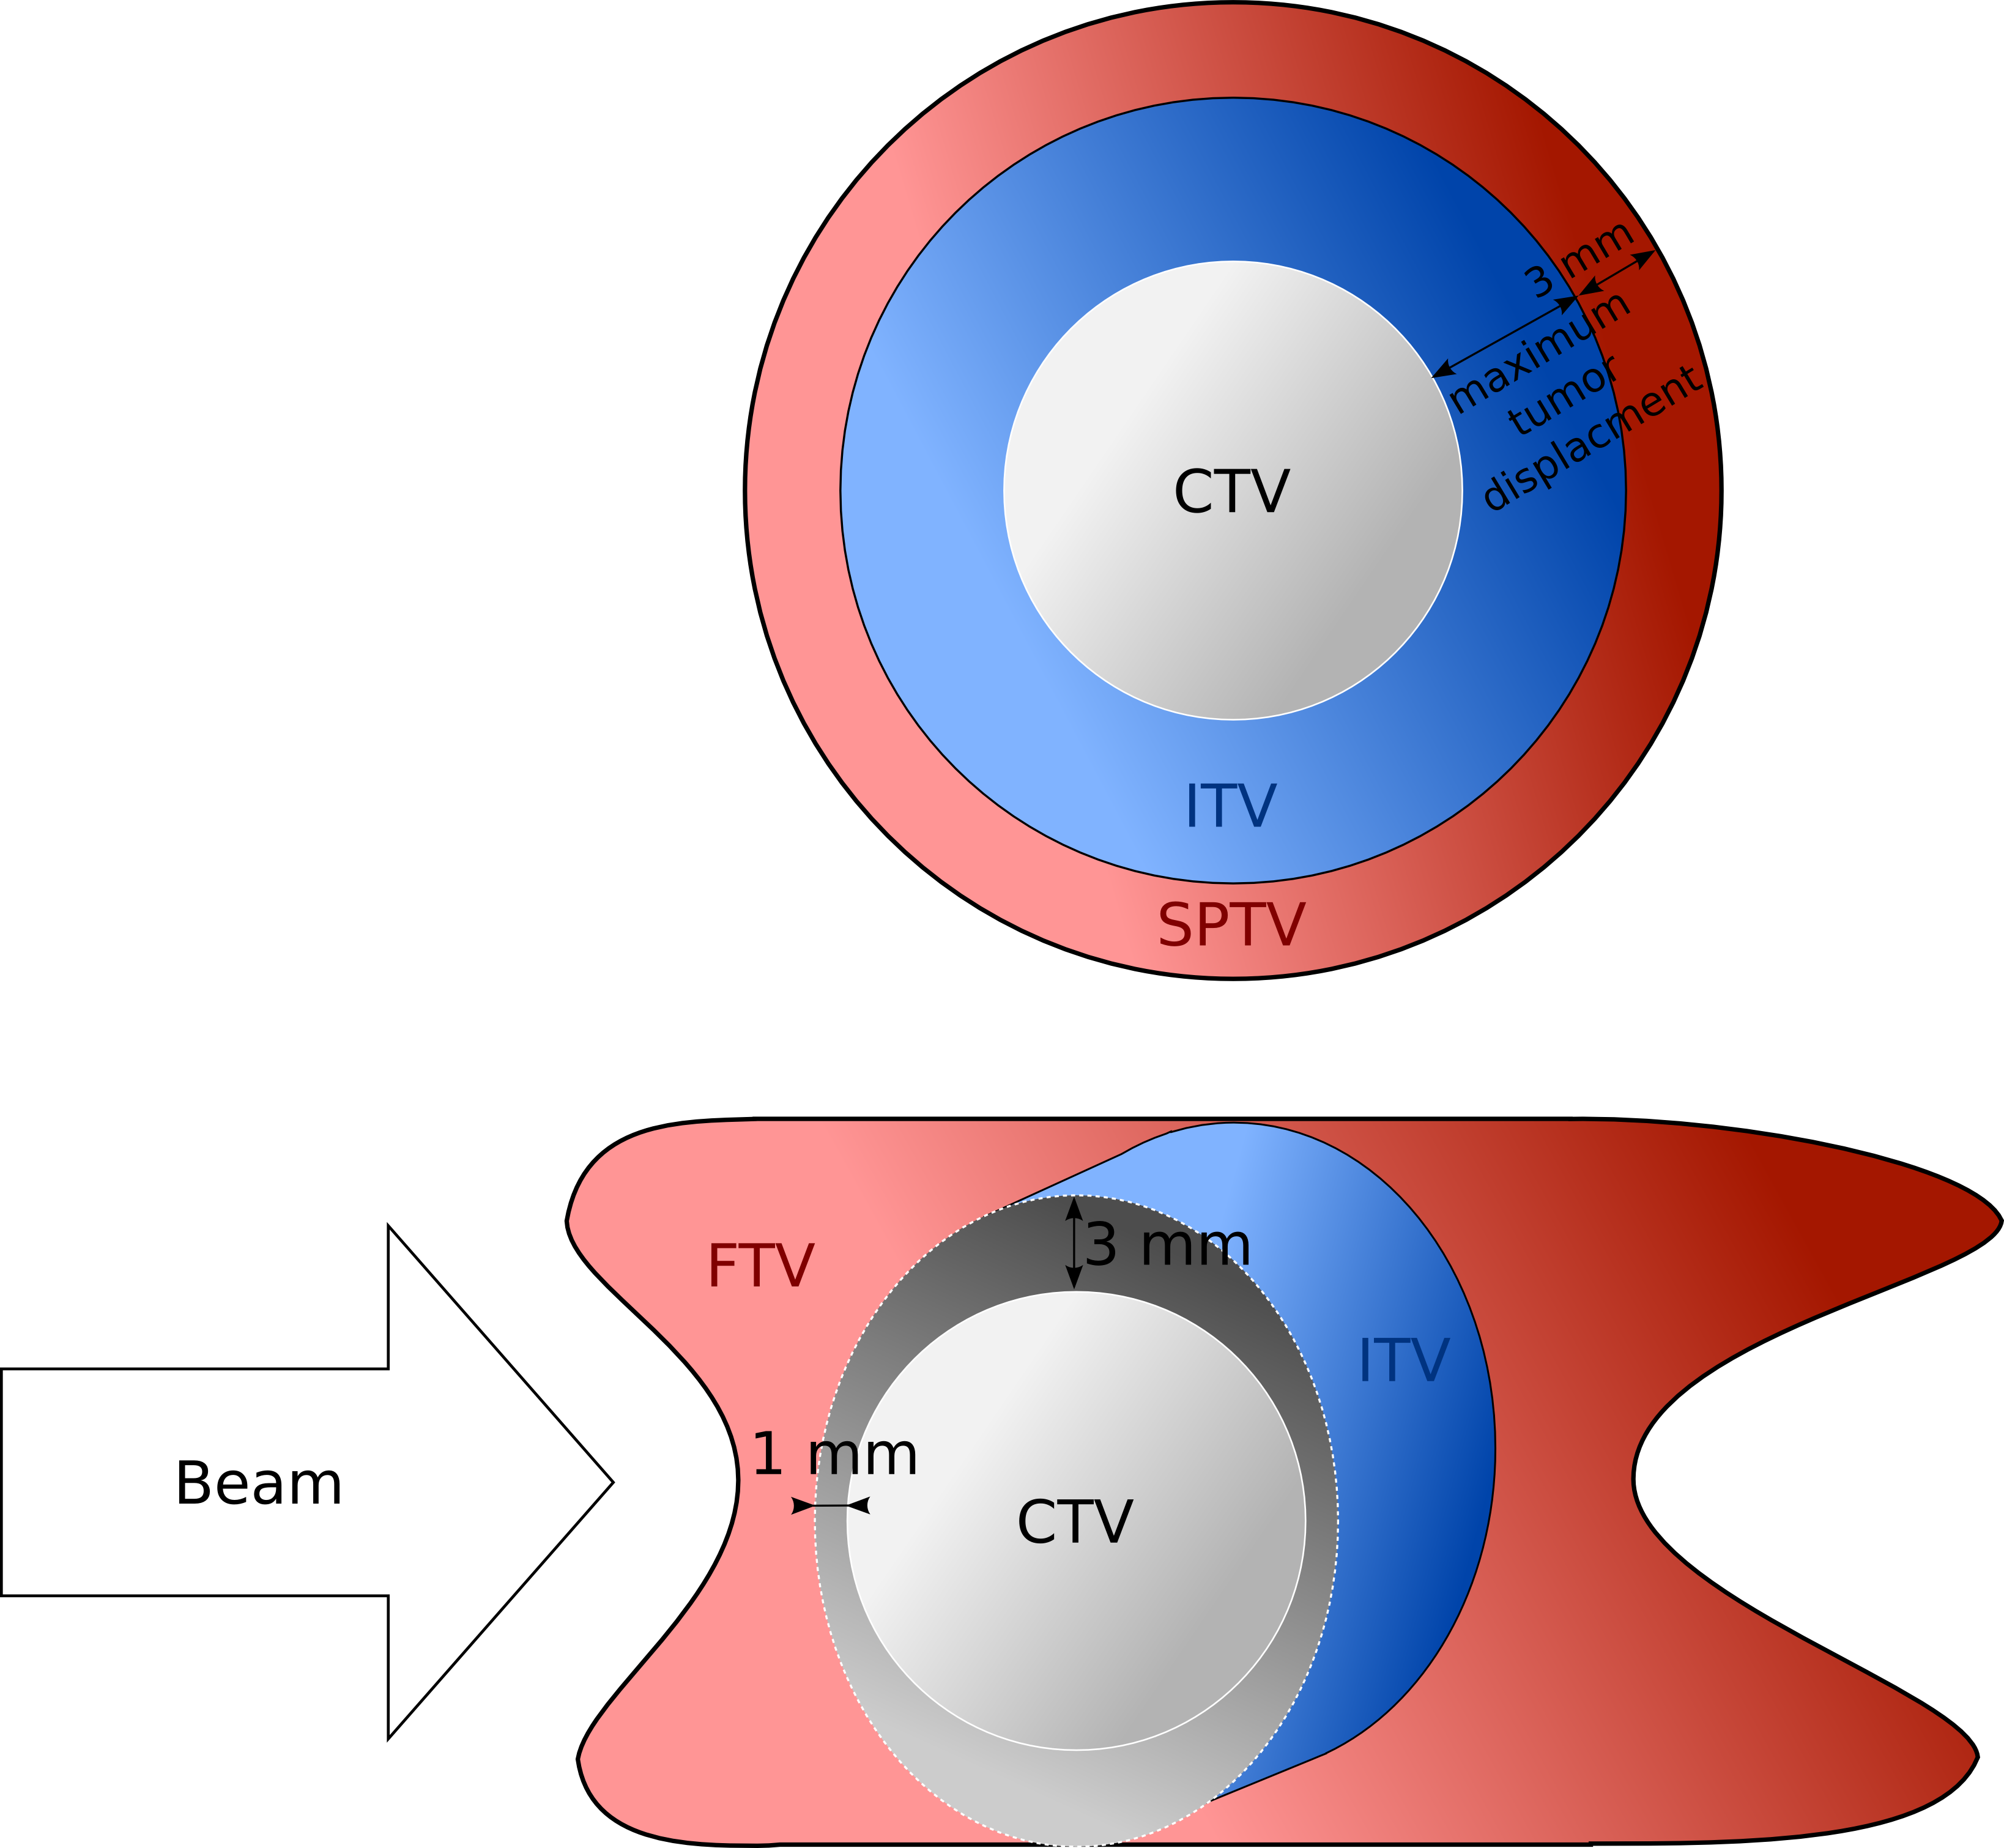
\includegraphics[width=0.9\textwidth]{./Images/PTV_definition.png}
\caption{Different PTV definitions for SDRT (SPTV) and CiT (FTV). For SPTV isotropic margins of 3 mm plus maximum tumor displacement due to 
breathing were used on the CTV; For FTV margins of 3 mm laterally and 1 mm in beam’s eye view were used and then range-ITV was constructed with
2 mm + 2\% range margins added for FTV in end-inhale phase.}
\label{Fig:PTV_def}
\end{center}
\end{figure}


\subsection{SDRT treatment planning}

The clinical plans were calculated with the Eclipse v10 planning system (Varian Medical Systems, Palo Alto, Ca, USA) using the AAA algorithm. All plans delivered 24 Gy, 
generally using 4 VMAT partial arcs. For tumor sizes $>$ 2.5 cm a calculation grid of 2.5 mm was used, otherwise it was 1 mm. During optimization, a first iteration included the 
SPTV only, after which the OARs were added. In order to lower OAR dose and improve the SPTV homogeneity,an artificial shell of 2 cm around the SPTV was created and the dose was minimized there as well.
Finally, an intermediate dose calculation with AAA was mandatory to get an adequate SPTV coverage after optimization.

\subsection{CiT treatment planning}

For CiT, state of the art 4D treatment planning software TRiP4D was used (see section \textbf{REF}). A single field uniform dose plan (SFUD) was optimized on the FTV in the end-inhale reference phase of the 4D-CT. 
Dose was then calculated on end-inhale (3D-0\%) and end-exhale (3D-50\%) phases. 4D dose delivery was simulated over the whole breathing cycle with two different breathing periods (3.6 and 5 s) and two different 
starting phases (0° and 90°). Simulations without motion compensation (4D-interplay) and with slice-by-slice rescanning were performed (4D-rescans). Five rescans were used for the majority of targets (n=24), whereas 20 rescans 
were used for targets (n=2) where the interplay effects were too big to achieve a satisfactory target coverage. 

Dose was computed considering the relative biological effectiveness (RBE) following the local effect model (LEM) IV \cite{Elsaesser2010}. The Alpha beta ratio was chosen conservatively, withion a ratio of 10 Gy
and 2 Gy for target and OARs, respectively. This led to RBE of approximately 1.1 in target tissue and approximately 1.1 to 3 in OARs. An example RBE distribution is shown in Fig.~\ref{Fig:RBE}

Most targets (n=20) were planned with two fields. For remaining targets, one (n=1), three (n=3) or four (n=2) fields were used due to proximity of OARs.
A beam spot spacing of 2 mm, a focal size of approximately 6 mm (FWHM), a 3 mm ripple filter and in most cases a bolus of a 80 mm width were used.

\begin{figure}[H]
\begin{center}
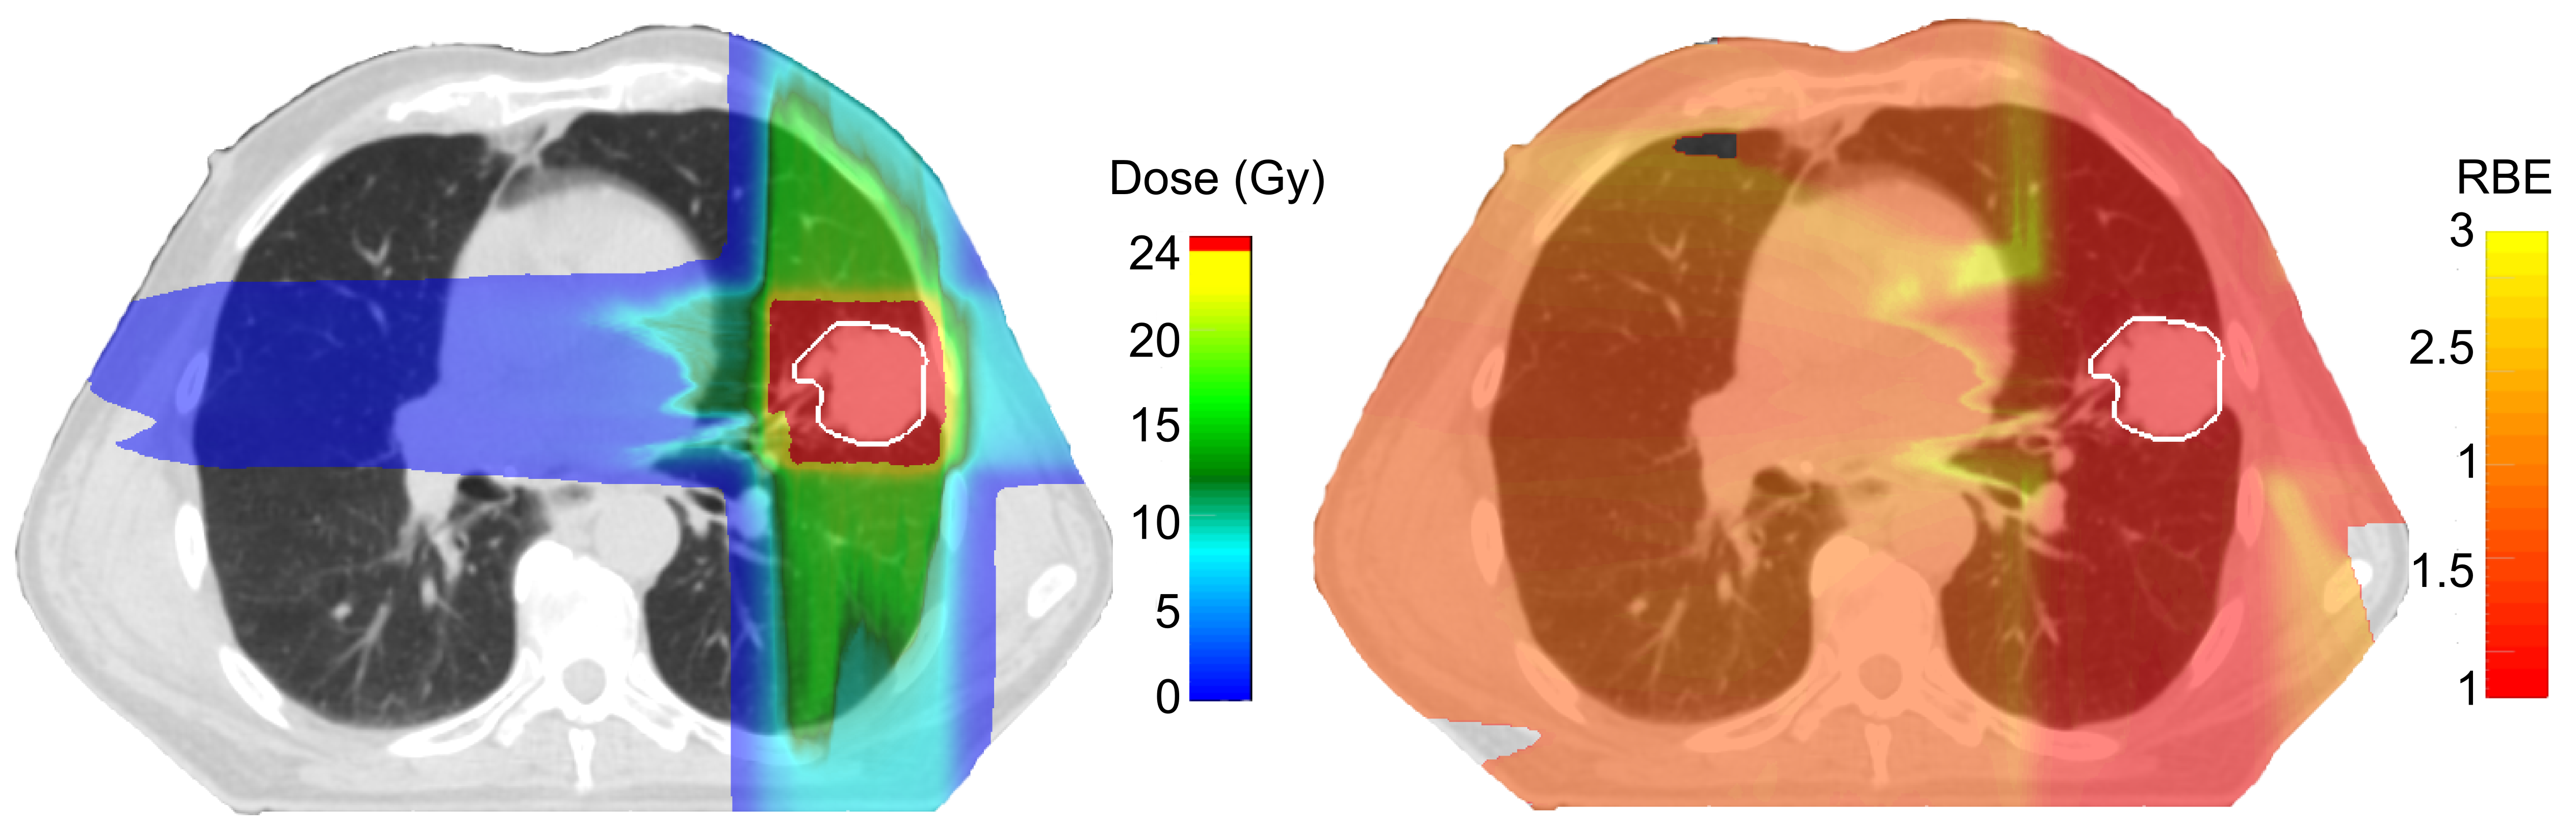
\includegraphics[width=0.9\textwidth]{./Images/RBE.png}
\caption{RBE distribution in a patient (a) depends on a actual dose profile (b).}
\label{Fig:RBE}
\end{center}
\end{figure}

\subsection{Dose metrics and analysis}


For comparison between SDRT and CiT the following dose metrics were used: a relative volume of the CTV receiving 100 \% of prescribed dose ($V_{100\%}$), 
the minimum dose in 95\% of the volume ($D_{95\%}$), the maximum point dose ($D_{Max}$), and the mean dose ($D_{Mean}$). The first two metrics, $V_{100\%}$ and $D_{95\%}$ were used 

to compare target coverage, whereas OAR dose was compared with DMax and DMean.

For 4D CiT dose calculations, mean and standard deviation were calculated for different breathing periods and starting phases.

Paired t-tests were performed to compare the dose metrics and for post-hoc exploratory analysis between groups a two-sided t-test with Welch correction for different variances
as carried out. A p-value < 0.05 was considered significant. Dose differences are always reported such that higher dose levels for SDRT result in positive values.

\section{Results}

Examples of two SDRT and 4D-rescan CiT treatment plans are shown in Figure~\ref{Fig:TreatmentPlans}. Patient A has two lesions in close proximity to the spinal cord. 
Patient B has a small lesion (0.87 cm$^3$) in the superior position of the left lung wing. $V_{100\%}$ is 100\% for SDRT and CiT in all CTVs for Patient A and B; 
average OAR difference between SDRT and CiT in $D_{Max}$ is 5.3 Gy and 1.5 Gy and in $D_{Mean}$ 1.2 Gy and 0.6 Gy, respectively for patient A and B.

\begin{figure}[H]
\begin{center}
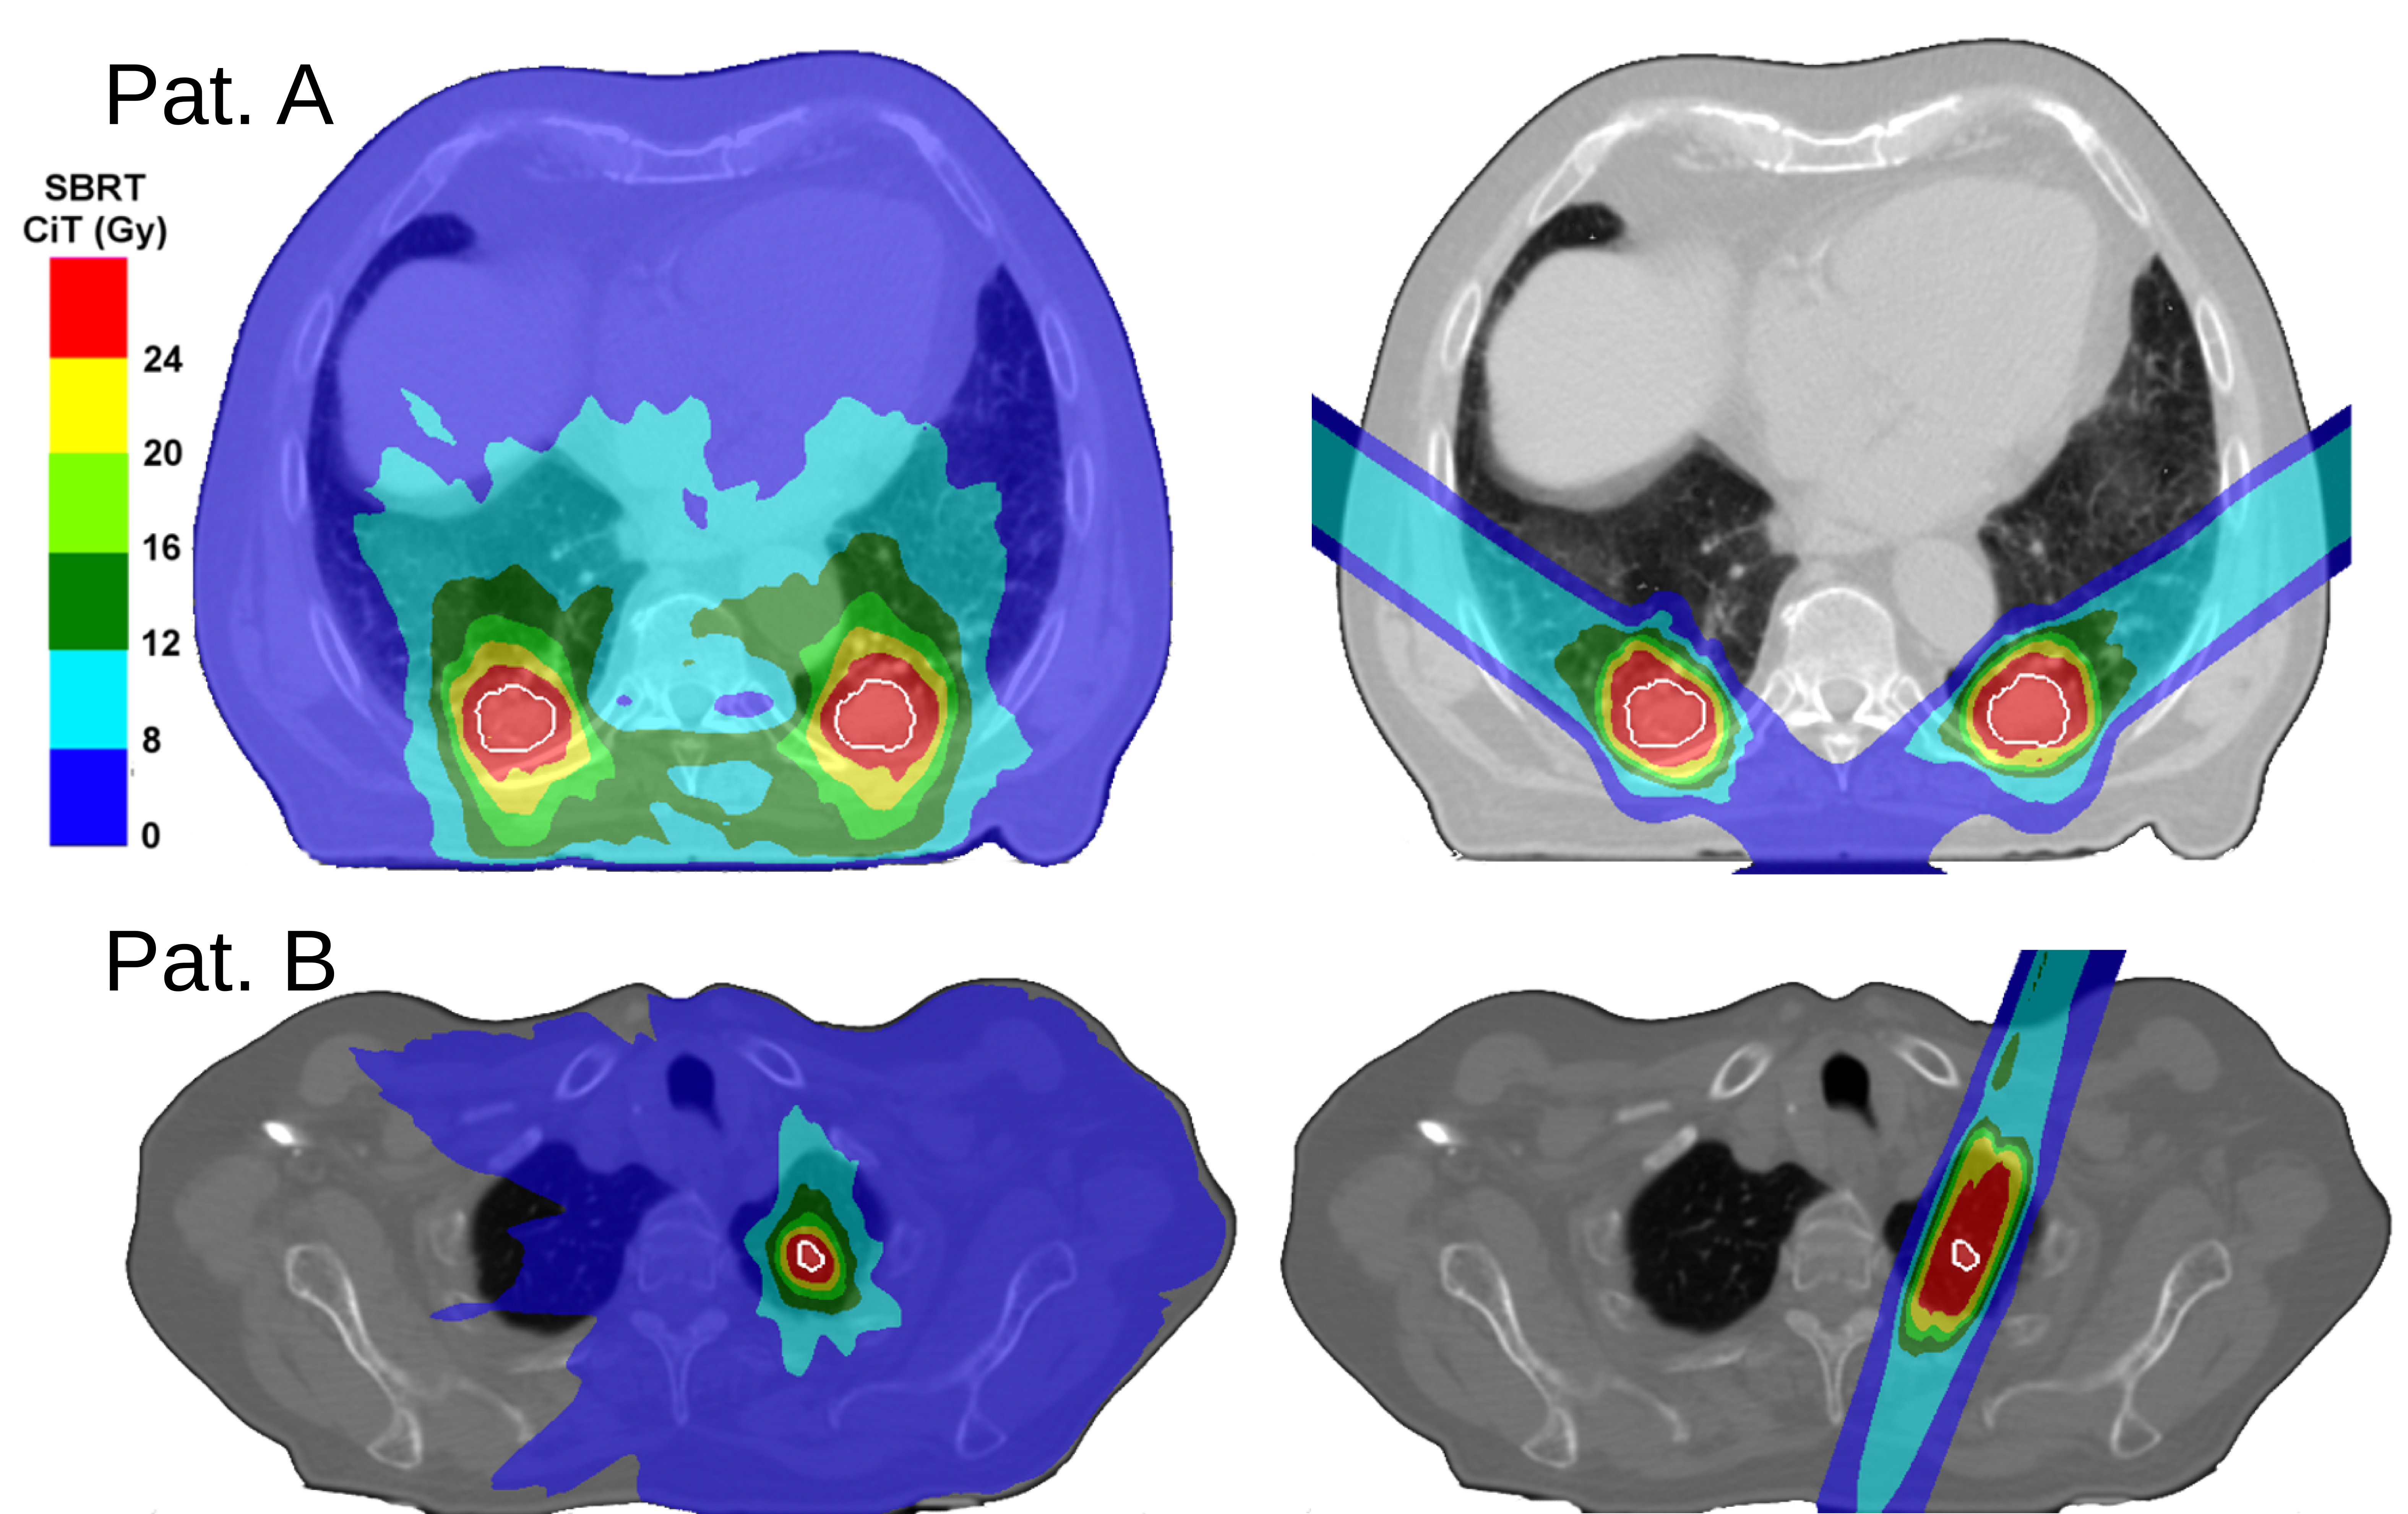
\includegraphics[width=0.9\textwidth]{./Images/TreatmentPlans.png}
\caption{Treatment plans for SDRT (left) and CiT (right) for two patients. 
Patient A (top row) might be better suited for CiT and patient B (lower row) for SDRT. The CTV contour is outlined in white.}
\label{Fig:TreatmentPlans}
\end{center}
\end{figure}

\subsection{Target Coverage}

Difference in PTV definition resulted in 1.5 (1.3 – 2.1) times bigger FTV than SPTV. There was no significant difference in CTV $D_{95\%}$ between SBRT and any CiT calculation. 
For CTV $V_{100\%}$ there was a significant difference between SDRT and 4D-interplay, 3.8 (0 – 6.1)\% and no significant difference between SDRT and 3D-0\%, 3D-50\% or 4D-rescan. 
Difference in V100\% between 4D-rescan and 4D-interplay with respect to CTV peak-to-peak motion and average CTV range change in water is plotted in Figure~\ref{Fig:InterplayDiff}. Range change was a 
better predictor of the  $V_{100\%}$ difference than geometric motion (r=0.75 vs. r=0.48).
There was a significant difference in  $V_{100\%}$ standard deviation between 4D-interplay and 4D-rescans, 1.8 (0 – 2.9)\%, i.e. interplay simulation showed a larger variability in dose coverage in addition to the difference in averages.

\begin{figure}[H]
\begin{center}
\includegraphics[width=0.9\textwidth]{./Images/InterplayDiff.png}
\caption{Difference in $V_{100\%}$  between 4D-interplay and 4D-rescan 
with respect to CTV peak-to-peak motion (black) and average CTV range 
change in water (red). Lines represent linear fit to data. Both lines have significant r (p < 0.05).}
\label{Fig:InterplayDiff}
\end{center}
\end{figure}

\subsection{Dose in OARs}

There was no significant difference in dose to OAR between the different CiT dose calculations. The dose metrics for SDRT and 4D-rescan CiT for 
OARs heart, spinal cord, smaller airway esophagus, trachea, aorta, ipsi- and contralateral lung are presented in Table~\ref{tab:results}. 
In almost all patients CiT deposited less dose in all OARs, except ipsilateral lung, where there was no statistical significant difference between SDRT and CiT. 
The average OAR difference between SDRT and CiT was significant, 2.5 (0.3- 4.8) Gy for $D_{Max}$ and 0.6 (0.2- 1.7) Gy for $D_{Mean}$. 
The contralateral lung did not receive any dose in 12 (71\%) patients with CiT.

\begin{table}[H]
  \centering
%   \footnotesize
  \caption{Dose metrics for OARs. First value at each organ is from SDRT and the second from 4D-rescan. All values are shown as median and 25-75\% in brackets.}
  \begin{tabular}{l|c|c|c|c|}
    \cline{2-5}
     & \multicolumn{2}{|c|}{$D_{Max}$ (Gy)} & \multicolumn{2}{|c|}{$D_{Mean}$ (Gy)} \\
     \hline
    \multicolumn{1}{|l|}{OAR} & Photon & Carbon & Photon & Carbon	\\
    \hline
\multicolumn{1}{|l|}{Heart} & 15.0 (11.9 - 21.8) & 10.8 (3.3 - 13.2) & 1.3 (0.1 - 2.2) & 0 (0 - 0.2)	\\
\multicolumn{1}{|l|}{Spinal Cord} & 9.3 (8.7 - 10.4) & 0 (0 - 5.9) & 0 (0 - 0.3) & 0 (0 - 0)	\\
\multicolumn{1}{|l|}{Smaller Airways} & 15.0 (13.4 - 20.2) & 10.9 (1.9 - 13.5) & 2.8 (1.5 - 5.8) & 0.7 (0 - 1.9)	\\
\multicolumn{1}{|l|}{Esophagus} & 11.0 (9.0 - 12.6) & 0 (0 - 0.7) & 1.1 (0.6 - 1.5) & 0 (0 - 0)	\\
\multicolumn{1}{|l|}{Aorta} & 19.3 (10.1 - 25.5) & 7.5 (2.0 - 14.3) & 1.4 (0.7 - 1.6) & 0 (0 - 0.1)	\\
\multicolumn{1}{|l|}{Ipsilateral Lung} & 26.3 (26.0 - 26.5) & 26.3 (25.8 - 26.8) & 2.3 (1.5 - 3.1) & 2.5 (1.6 - 3.4)	\\
\multicolumn{1}{|l|}{Contralateral Lung} & 4.8 (3.5 - 6.8) & 0 (0 - 0.3) & 0.4 (0.2 - 0.6) & 0 (0 - 0)	\\
    \hline\hline
  \end{tabular}
  \label{tab:results}
\end{table}

\subsection{Dependence on CTV Size}

Significant differences were observed between patients with a single CTV smaller (n=8) or larger (n=7) than 2.5 cm$^3$ for
$D_{Max}$ and $D_{Mean}$, see Figure~\ref{Fig:OAR_boxplots}. For patients with a smaller CTV, the dosimetric advantage over SDRT was on average 1.3 Gy and 0.5 Gy lower for DMax and DMean, respectively. 
This was associated with FTV definition - the average volume ratio between FTV and SPTV was 2.9 (1.6 – 4.0) and 1.5 (1.3 – 1.8), for patients with CTV < 2.5 cm$^3$ and CTV > 2.5 cm$^3$, respectively
Patients with multiple lesions were excluded in this comparison. The DMax and DMean difference were on average higher in these patients, but the number of patients was too low for statistical analysis. 

\begin{figure}[H]
\begin{center}
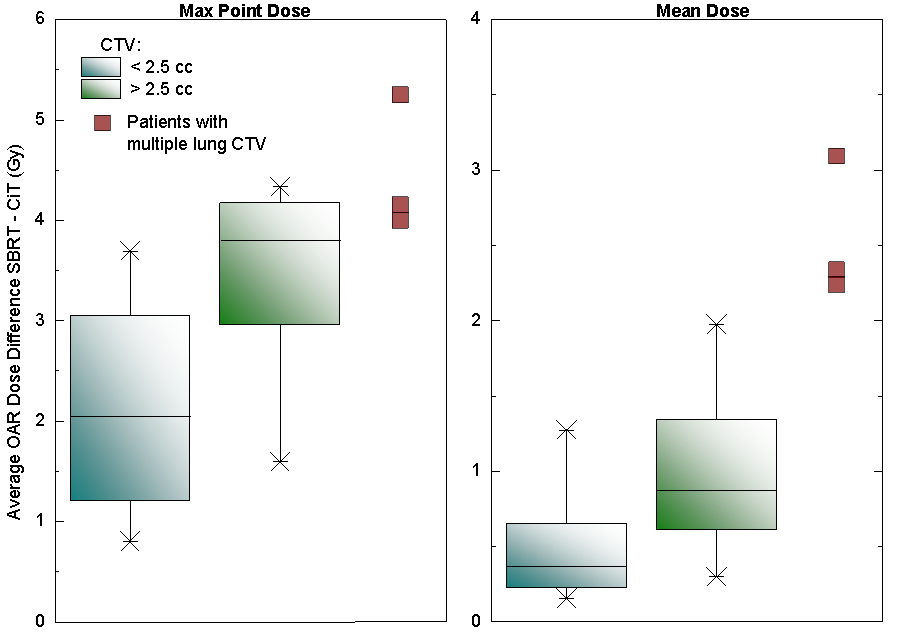
\includegraphics[width=0.9\textwidth]{./Images/OAR_boxplots.png}
\caption{Box plots of average OARs $D_{Max}$ and $D_{Mean}$ difference between SDRT and CiT for patients with
single CTV smaller (n = 8) or bigger (n = 7) than 2.5 cm$^3$. Boxes represent 25\% - 75\%, 
whiskers 10\% - 90\% of data, median is shown with solid line and outliers with crosses. 
Values for patients with multiple lung lesions are shown with square symbols.}
\label{Fig:OAR_boxplots}
\end{center}
\end{figure}


\section{Discussion}

This is the first in silico study directly comparing clinically valid SDRT (or SBRT) plans to scanned carbon ion plans using state of the art 4D dose calculation and 
motion mitigation methods for NSCLC patients. Our study found that CiT deposited less dose to OARs compared to SDRT. Therefore CiT might be considered as an alternative 
treatment option to SDRT. The finite range of the beam permits a small number of fields and thus a narrow entry channel, so that critical OARs such as spinal cord, 
heart, esophagus, and the contralateral lung could be effectively spared using CiT, with typically low or even zero dose. CiT could be thus highly beneficial 
to patients with impaired contralateral lung function, because CiT deposited no dose in the contralateral lung in 11 patients, while SDRT irradiated the contralateral
lung in all patients. Being an intensity-modulated arc therapy, SDRT had an advantage in some patients where the smaller airways were in a close proximity to CTV; 
SDRT could shape the dose distribution to reduce dose to the smaller airways, compensating CiT’s advantageous physical dose characteristics.

Further increase in OAR sparing could be achieved by using intensity modulated particle therapy (IMPT) instead of SFUD. While IMPT could lead to 
less dose in the OARs, it would make the plans less robust against the setup errors due to additional dose gradients between the fields. These gradients can be 
controlled by employing robust optimization to acm$^3$ount for range, motion and setup uncertainties, which we will implement in a future 4D treatment planning study \cite{Chen2012}.

\subsection{Range Margins and Motion Mitigation}

Since conventional geometric margins are not suitable for PT \cite{Park2012}, margins based on range changes were used. Another trial comparing photon to proton therapy in
NSCLC patients also used different PTV definitions to incorporate range changes \cite{Roelofs2012}. As shown in our study, inclusion of range changes leads to increase in FTV,
up to 4.7 times compared to SPTV. Furthermore, the difference between PTVs is bigger for smaller tumor sizes. Patients with bigger tumor volumes (CTV > 2.5 cm$^3$) 
are therefore better suited for treatment with CiT. 

Our results confirm previously published results that interplay can lead to a dose degradation in treating moving targets with active scanned beam \cite{Bert2008}. 
Fig.~\ref{Fig:InterplayDiff} shows the importance of using 4D dose calculation and motion mitigation techniques in treating moving targets. Even small motions and/or range 
changes can lead to underdosage in CTV. While FTV appears a strong motion mitigation technique (no difference in CTV $D_{95\%}$ between SDRT and CiT), 
it is necessary to use rescanning as well to get sufficient target coverage (CTV $V_{100\%}$ = 100\%). Rescanning is also more robust to different breathing
periods and starting phases compared to 4D-interplay, indicated by the lower variance in the dose coverage metrics. Recent studies suggest that some 
patients require phase-controlled layer or volumetric rescanning for sufficiently robust target coverage \cite{Mori2013,Takahashi2014}. The advantage of slice-by-slice 
rescanning is that no motion monitoring or assumptions on the breathing frequency are necessary.

\subsection{Clinical results}

Grutters et al. have performed a meta-analysis on comparison between photon, proton and carbon ions in treating NSCLC \cite{Grutters2010}. They found similar 5-year 
survival rates for SBRT, protons and carbon-ions (around 40\%). However, the number of patients treated with particle therapy was low and they
advise caution when interpreting the data. Also different fractionation schemes were used in the comparison. A more recent review was published 
by Tsujii and Kamada where they reported a high 3-year survival rate for single-fraction carbon-ions (76.9\%) \cite{Tsujii2012}. In comparison, SBRT had 55.8\% 
3-year survival rate [6]. Additionally, no late treatment-related adverse effects were reported for carbon-ions, whereas in SBRT grade 3 was observed 
in up to 28\% of patients. All patient data for PT was based only on passively scattered beam, but first patients are treated in thoracic and 
abdominal regions with an active beam scanning at the National Institute for Radiological Sciences (NIRS) in Japan \cite{Mori2013}.

\subsection{RBE and Proton Therapy}

Carbon ions exhibit a radiobiological advantage, especially in the Bragg peak region. However, for high doses as used here the effect of RBE is not well 
documented and is subject to ongoing research \cite{Friedrich2014}. For these high doses RBE for carbon ions should approach a value between 1 and 2 \cite{Carabe2007}, which is in 
agreement with values in our study (\~ 1.1).

Coincidently, RBE values in the target at high doses are similar to those used clinically in proton therapy. Our results are in agreement with several
in silico studies comparing SBRT and proton therapy for NSCLC \cite{Roelofs2012, Kadoya2010, Register2010}. Furthermore, a study made by Kadoya reached the same conclusion as our study,
that patient with larger CTV and/or multiple CTVs would benefit more from proton therapy \cite{Kadoya2010}. A recent phase II trial for patients with multiple sites 
of  extracranial disease showed very good results for photons \cite{Iyengar2014}. Based on our conclusions proton and/or carbon-ion therapy is a sensible treatment 
option. Carbon-ions shows considerably lower lateral scattering though, which should result in even better OAR sparing than protons.

\subsection{Study limitations}

The 4D dose calculations were based on a regular breathing pattern, which typically varies during patient treatment and/or between 4DCT acquisition 
and actual treatment \cite{Verma2010, Malinowski2011}. A possible solution was proposed by Boye et al. to get motion information from 4D magnetic resonance imaging (4DMRI)
and use it in 4D dose calculations \cite{Boye2013}.

Furthermore, SDRT treatment plans were done on a static case in contrast to a 4D dose calculation done for CiT. This should not influence the 
results of our study, since motion has a smaller impact on photon dose distributions \cite{Zou2014}, whereas it is imperative in CiT dose calculations \cite{Bert2011}. 

There were also differences in treatment planning. CiT plans were done by a single person in a research setting, whereas SDRT plans were made by
different people under clinical conditions with the requirement to finish the plans on time. 

Slight changes also existed between the planning CT, used for SDRT treatment plans and 4D-CT used for CiT treatment plans, even though 4D-CT was 
usually acquired right after the planning CT. The propagation of contours from the planning CT to the 4D-CT and also for the 4D dose calculation 
rely on deformable image registration (DIR), where even small changes can effect 4D dose distribution \cite{Kashani2008}. Results from deformable registration
were therefore thoroughly checked with different approaches, such as inspection of the warped image, evaluation of the Jacobian values and the 
inverse consistency of the vector field. However, the transformation of the dose with DIR is a debated topic and might jeopardize the simulated 
results, especially with respect to the 4D target coverage. On the other hand, dose differences in OARs were large and should be robust against 
vector field errors in the order a few mm. Nevertheless, further studies are warranted, possibly using advanced moving phantoms for an experimental 
validation \cite{Perrin2014}, and finally also clinical trials.

\subsection{Application}
Scanned carbon ion therapy is available only in a limited number of clinics, mainly due to the considerably higher cost in comparison to photon linacs.
Therefore a careful patient selection appears sensible. Patients with larger and multiple lesions where SDRT might be limited due to OAR constraints 
could be referred to carbon centers. In this study, already lesions larger than 2.5 cm$^3$ were found to benefit significantly stronger from CiT.


\bibliographystyle{apalike}
\bibliography{../ref.bib}{}

\end{document}